\graphicspath{ {./JiaweiZhuang/HW2_figures/basic_variables/} }

\begin{solution} 

The pressure is computed from

    \begin{align*}
        p &= c_s^2 \rho= \frac{1}{3} \rho
    \end{align*}

Fig \ref{fig:macro_case1} and Fig \ref{fig:macro_case2} show the macroscopic fields with the periodic (case 1) and non-periodic (case 2) boundary conditions.

\textbf{Periodic Boundary Conditions}

\begin{figure}[H]
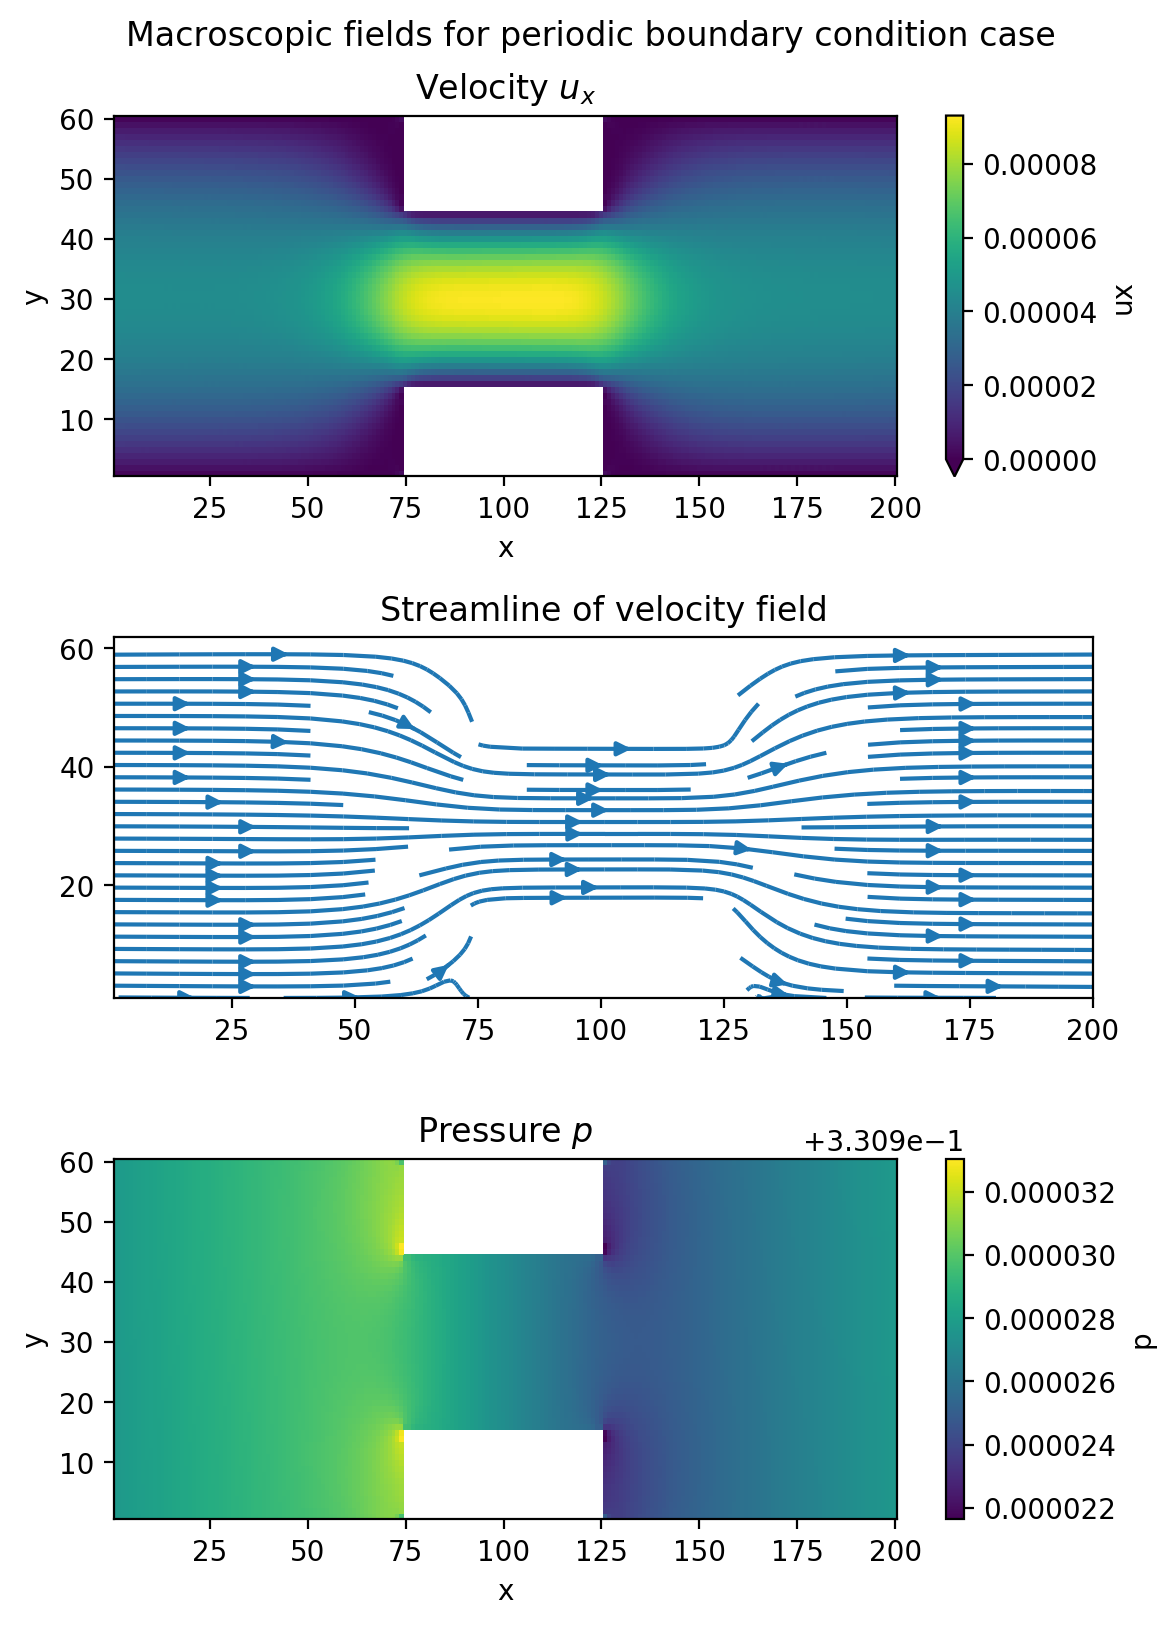
\includegraphics[scale=0.76]{case1_2d_fields}
\centering
\caption{Macroscopic variables for periodic boundary case}
\label{fig:macro_case1}
\end{figure}

\end{solution}

\begin{solution} 
\textbf{Imposed Boundary Conditions}

\begin{figure}[H]
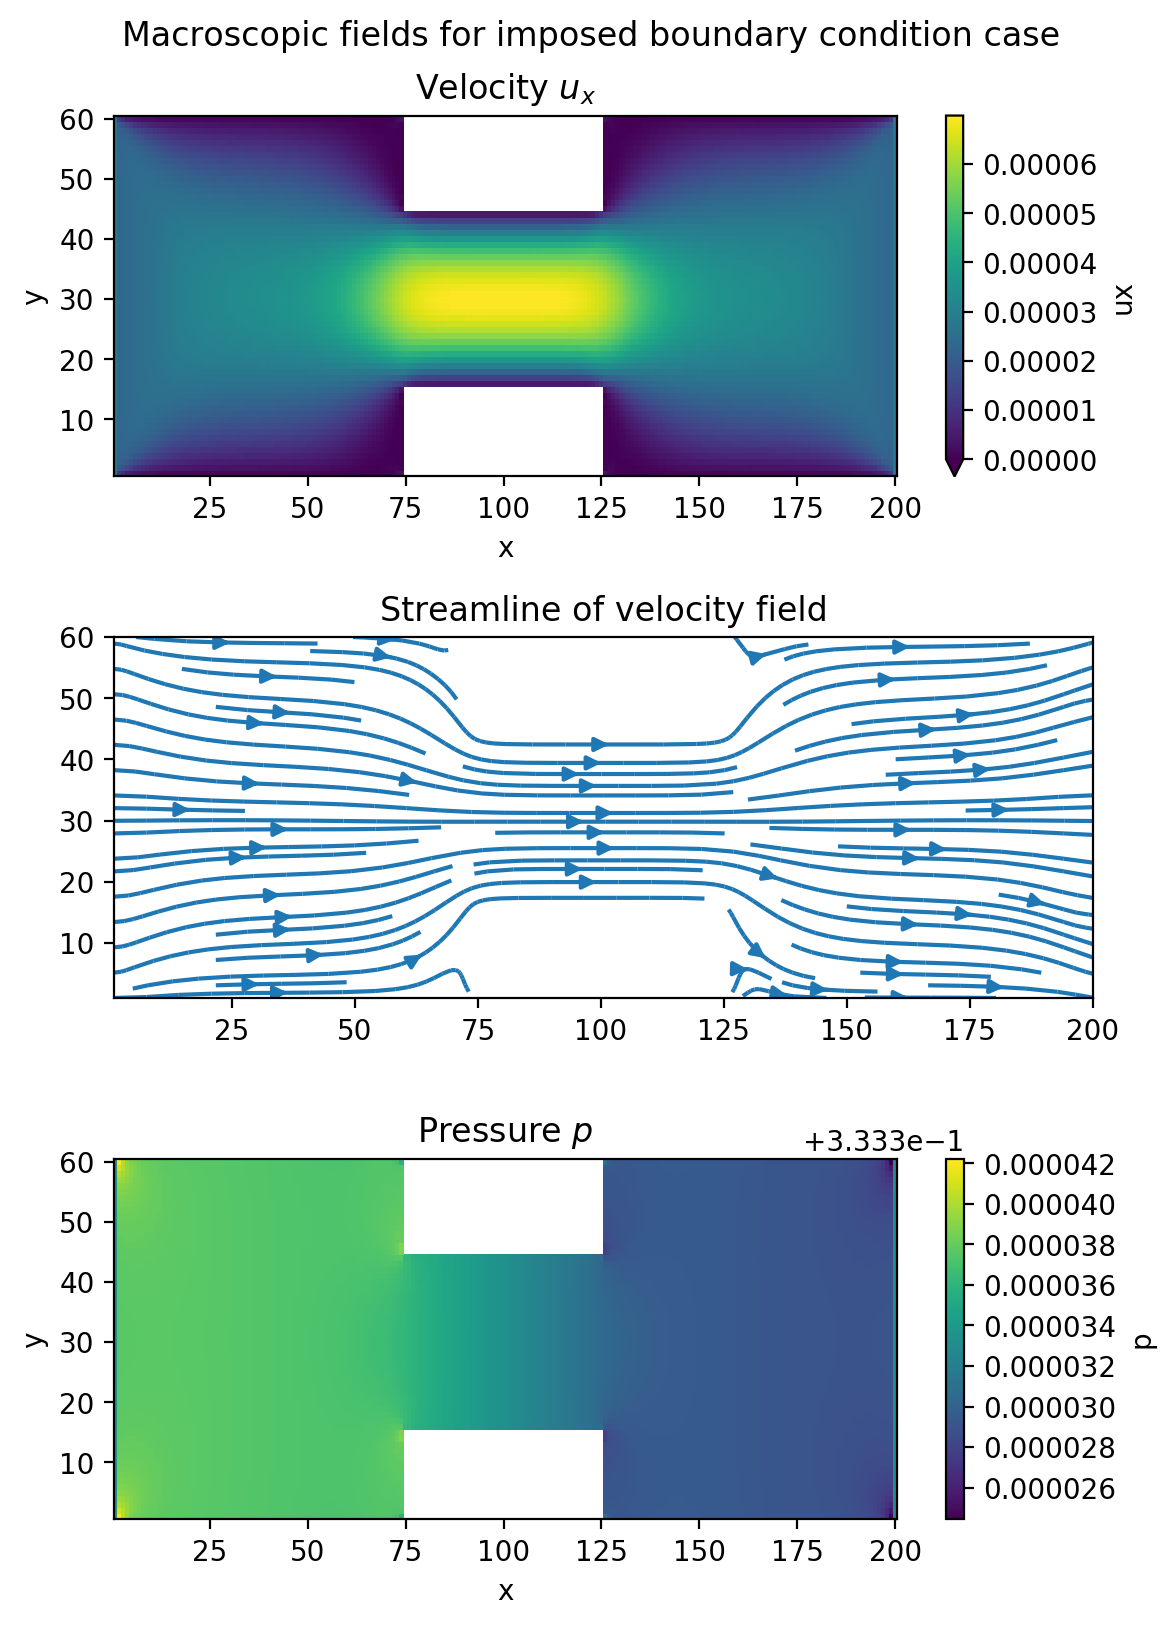
\includegraphics[scale=0.76]{case2_2d_fields}
\centering
\caption{Macroscopic variables for non-periodic boundary case}
\label{fig:macro_case2}
\end{figure}

\end{solution}

\begin{solution} 
\textbf{Volume Flow Rate}

The volume flow rates can be computed from the integral over x, on a specific cross-section $x=x_i$. Fig \ref{fig:flow_case1} and Fig \ref{fig:flow_case2} show the volume flow rate at all possible $x$, for two different boundary conditions. The rate is roughly constant at different $x$. For boundary case 1, $rate \approx 0.0018$; for boundary case 1, $rate \approx 0.0014$.

\begin{figure}[H]
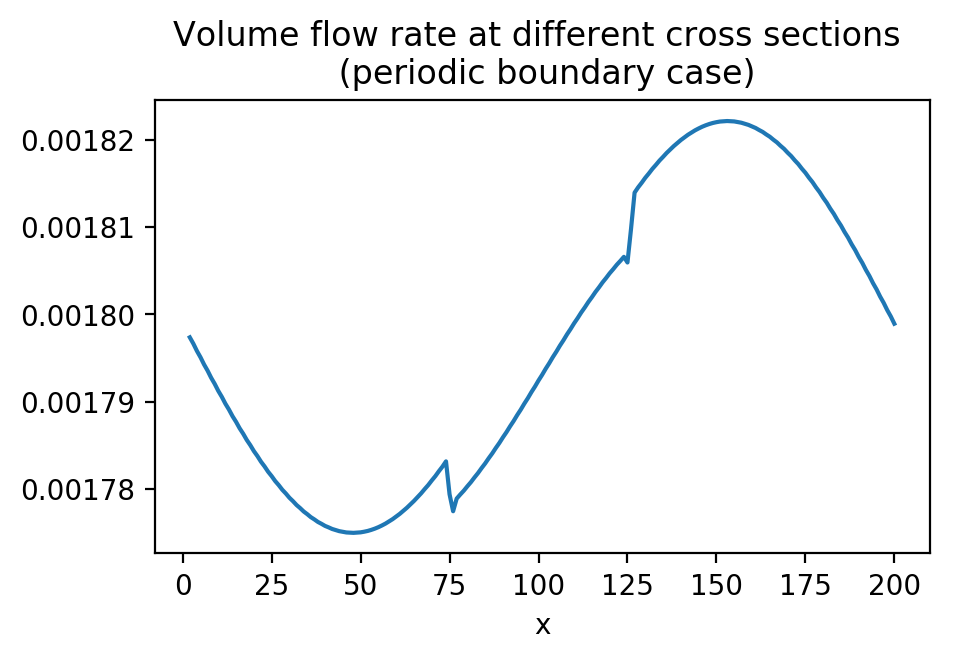
\includegraphics[scale=0.8]{case1_volume_flow}
\centering
\caption{Volume flow rates for periodic boundary case}
\label{fig:flow_case1}
\end{figure}

\begin{figure}[H]
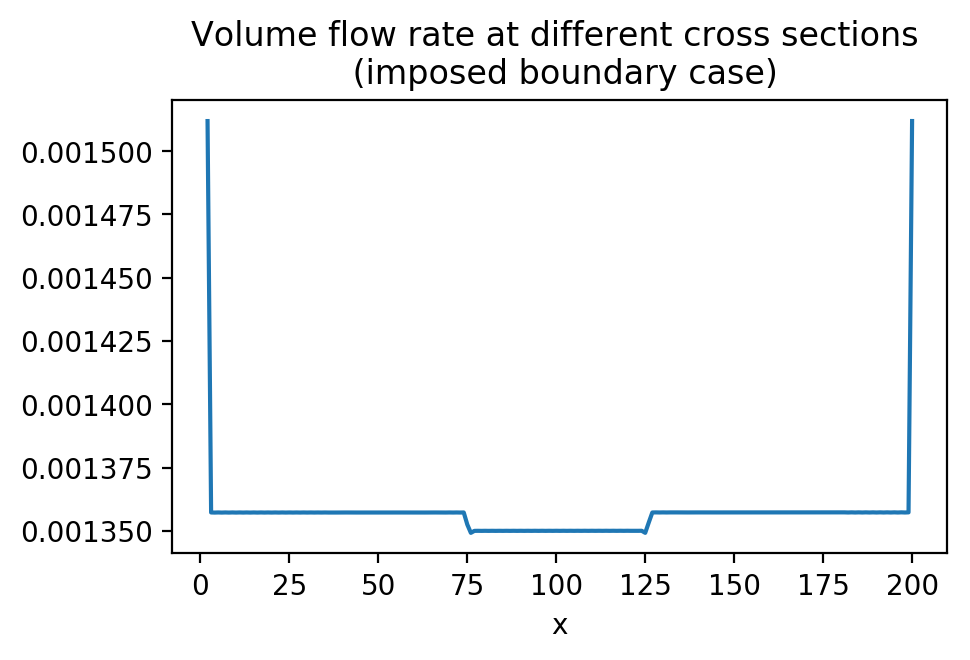
\includegraphics[scale=0.8]{case2_volume_flow}
\centering
\caption{Volume flow rates for non-periodic boundary case}
\label{fig:flow_case2}
\end{figure}

\end{solution}

\begin{solution} 
\textbf{Average Velocity}

The average velocity is $3.45 \times 10^{-5}$ for periodic boundary and $2.61 \times 10^{-5}$ for non-periodic. 

The maximum velocity is $9.30 \times 10^{-5}$ for periodic boundary and $6.98 \times 10^{-5}$ for non-periodic. $u_y$ is orders of magnitude smaller than $u_x$ and has negligible contribution to the total velocity magnitude.

We can further plot the average and maximum velocity at each cross-section $x=x_i$, as shown in Fig \ref{fig:profile_case1} and Fig \ref{fig:profile_case2}. This velocity is significantly higher inside the narrowing region, consistent with the continuity equation of fluid. This result also matches our intuition of the system.

\begin{figure}[H]
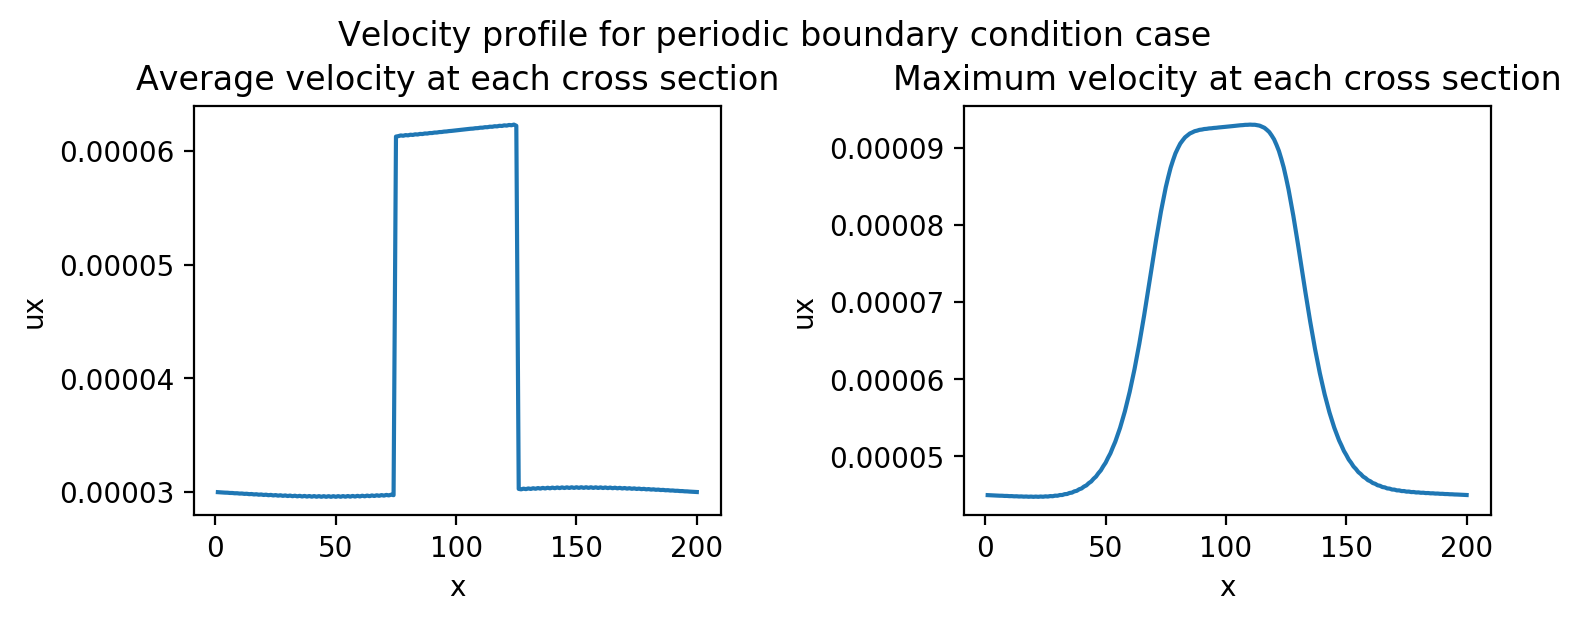
\includegraphics[scale=0.75]{case1_u_profile}
\centering
\caption{Average and maximum velocity at each cross-section, for periodic boundary case}
\label{fig:profile_case1}
\end{figure}

\begin{figure}[H]
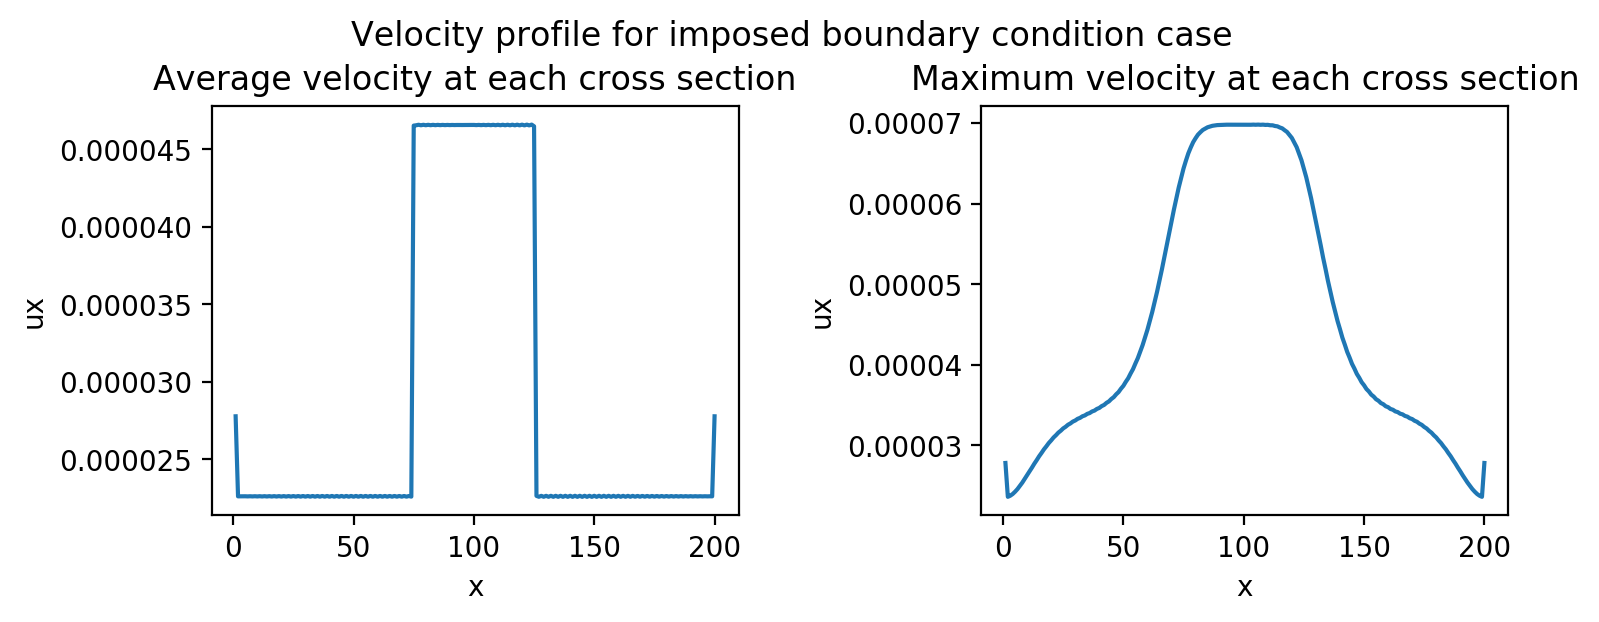
\includegraphics[scale=0.75]{case2_u_profile}
\centering
\caption{Average and maximum velocity at each cross-section, for non-periodic boundary case}
\label{fig:profile_case2}
\end{figure}

\end{solution}

\begin{solution} 

We can further check the velocity profile at each cross-section. For 2D Poiseuille flow without walls, the analytical solution is known to be a parabola. With walls, the shape should still be parabola-like, as confirmed by Fig \ref{fig:profile_case1} and Fig \ref{fig:profile_case2}. Inside the narrowing region ($x=100$), the parabola is the sharpest. The only non-parabola-like profile is the non-periodic boundary case at $x=0$, because we impose uniform velocity at the boundary.

\begin{figure}[H]
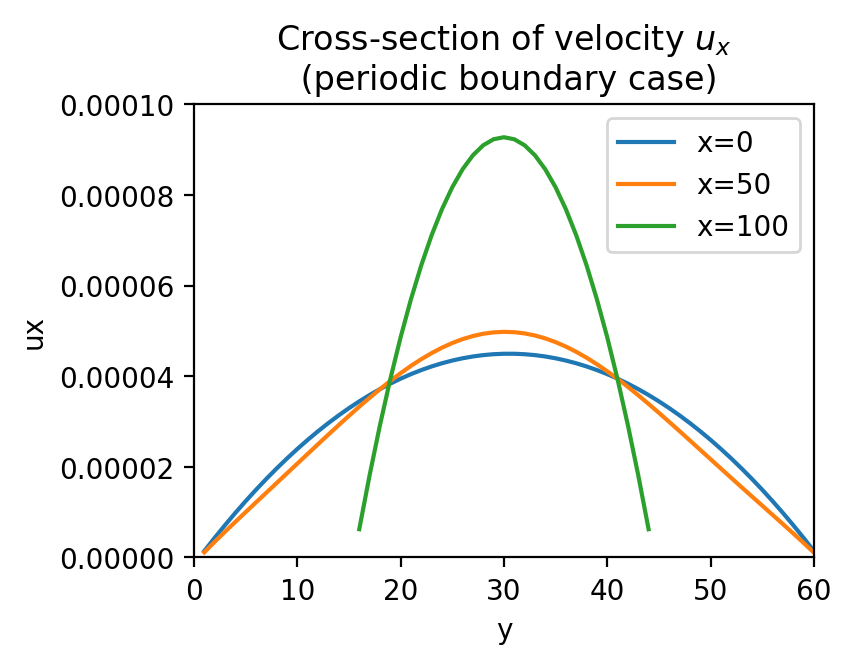
\includegraphics[scale=0.75]{case1_u_cross_section}
\centering
\caption{Velocity profile at three cross-sections, for periodic boundary case.}
\label{fig:profile_case1}
\end{figure}

\begin{figure}[H]
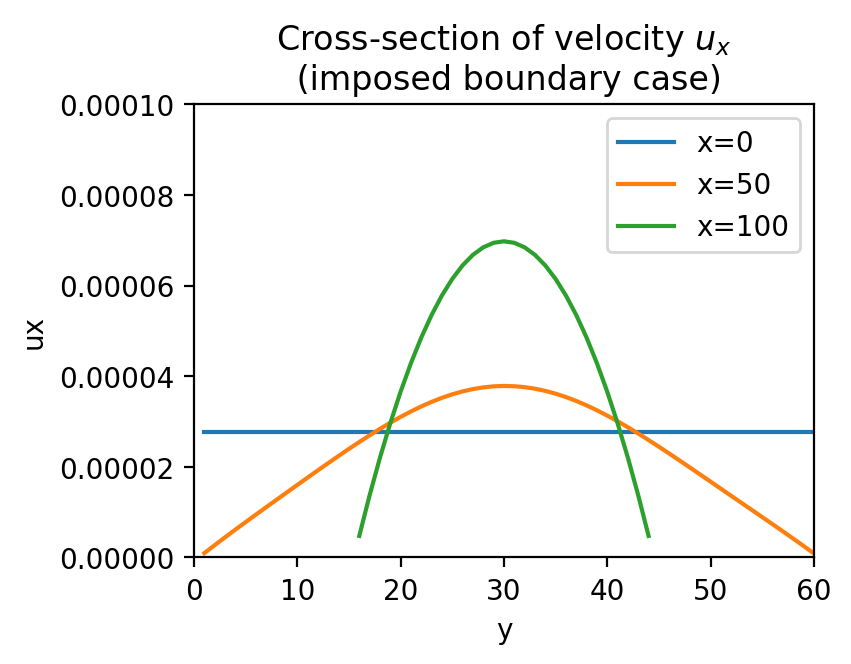
\includegraphics[scale=0.75]{case2_u_cross_section}
\centering
\caption{Velocity profile at three cross-sections, for non-periodic boundary case.}
\label{fig:profile_case2}
\end{figure}

\end{solution}

